\documentclass[12pt,a4paper]{article}
\usepackage[utf8]{inputenc}
\usepackage[english]{babel}
\usepackage{graphicx}
\usepackage{amsmath}
\usepackage{amssymb}
\usepackage{geometry}
\usepackage{hyperref}
\usepackage{xcolor}
\usepackage{booktabs}
\usepackage{enumitem}
\usepackage{float}
\usepackage{caption}
\usepackage{colortbl}
\captionsetup{font=small,labelfont=bf}
\usepackage{subcaption}

% Set page margins
\geometry{margin=1in}

% Define colors
\definecolor{myblue}{RGB}{0,102,204}
\definecolor{mygreen}{RGB}{0,153,0}
\definecolor{myred}{RGB}{204,0,0}

% Title
\title{
\vspace{-1.5cm}

\includegraphics[width=0.4\textwidth]{YULogo.png}\\
\vspace{1cm}
{\LARGE\textbf{IoT Architectures, Protocols and Security (NES424)}}\\
\vspace{0.5cm}
{\Large Assignment}\\
\vspace{0.3cm}
{\large Spring 2025 Semester}
}

\author{%
\begin{tabular}{|l|l|}
\hline
\textbf{Student Name} & \textbf{Student ID} \\
\hline
Khaled Alanbar & 202211365 \\
\hline
Rian Bawazir & 202111145 \\
\hline
Ali Bawazir & 202211018 \\
\hline
\end{tabular}%
\vspace{0.5cm}%
}
\date{\today}

\begin{document}

\maketitle
\thispagestyle{empty}

\begin{center}
\textbf{Submitted to:} Prof. Sanaa Ghouzali
\end{center}

\vspace*{\fill}

\begin{center}
\fbox{\parbox{0.9\textwidth}{
\textbf{OBJECTIVE:} The goal of this assignment is to engage students in exploring IoT devices and systems used in smart agriculture, smart cities, and healthcare. Students will research an IoT device and design a corresponding IoT system architecture, considering the IoT architectural drivers, communication criteria, and data management strategies.
}}
\end{center}

\vspace*{\fill}

\newpage
\section{IoT Device Research}

\subsection{Soil Moisture Sensor for Smart Agriculture}

\subsubsection{Device Overview}

\begin{figure}[H]
\centering
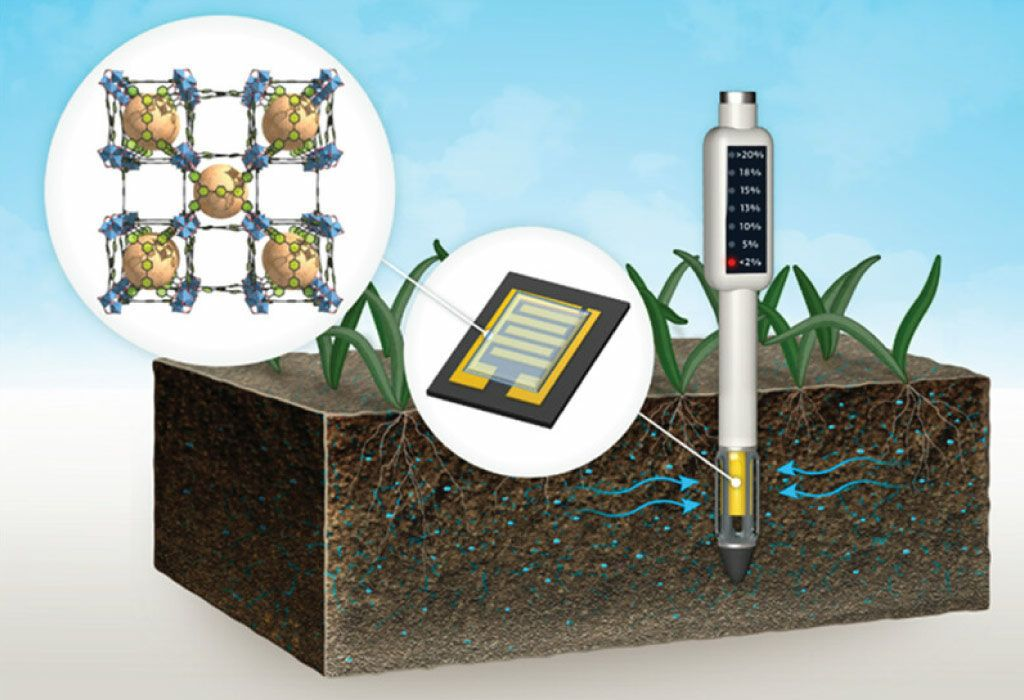
\includegraphics[width=0.7\textwidth]{img/soil_moisture_sensor.jpeg}
\caption{Soil Moisture Sensor Illustration}
\label{fig:soil_moisture_sensor}
\end{figure}

The selected IoT device is a soil moisture sensor designed specifically for smart agriculture applications. This sensor measures the volumetric water content in soil, providing farmers with real-time data about soil conditions. The device consists of two main components: the sensing probes that are inserted into the soil and the transmitter module that processes and sends the data.

The sensor operates on the principle of electrical conductivity, where water acts as a conductor of electricity. When soil is wet, it conducts more electricity (lower resistance), and when dry, it conducts less electricity (higher resistance). The sensor quantifies this resistance and converts it into a soil moisture percentage value, typically ranging from 0\% (completely dry) to 100\% (saturated).

Most modern agricultural soil moisture sensors are equipped with temperature sensors as well, providing additional context to the moisture readings, as temperature affects water availability to plants. The device used in this application utilizes LoRaWAN protocol for data transmission, which is ideal for agricultural settings where power infrastructure may be limited and long-range communication is necessary.

\subsubsection{Application Area}
This soil moisture sensor is utilized in precision agriculture, specifically in an automated irrigation system for large-scale wheat farming in arid regions. The implementation works as follows:

\begin{itemize}
    \item Multiple sensors are strategically placed across different zones of the farm, considering soil variations, topography, and crop density.
    \item Each sensor takes readings at predefined intervals (typically every 30 minutes) and transmits the data to a central gateway.
    \item The system analyzes the collected data against predefined moisture thresholds specific to wheat crops and their growth stages.
    \item When soil moisture falls below the optimum level, the system automatically triggers irrigation in the specific zones that need water, rather than watering the entire field uniformly.
    \item Farmers can access real-time and historical soil moisture data through a mobile application or web interface, allowing them to make informed decisions about water management.
\end{itemize}

This targeted approach significantly reduces water usage while optimizing crop yield, as each section of the field receives precisely the amount of water it needs.

\subsubsection{Benefits and Challenges}

\textbf{Benefits:}
\begin{itemize}
    \item \textbf{Water Conservation}: The precise monitoring enables targeted irrigation, reducing water usage by up to 30-50\% compared to traditional methods.
    \item \textbf{Improved Crop Yield}: By maintaining optimal soil moisture conditions, plants experience less stress, resulting in better growth and higher yields.
    \item \textbf{Labor Reduction}: The automated system eliminates the need for manual soil checking and irrigation adjustments, saving significant labor costs.
    \item \textbf{Data-Driven Decisions}: Historical moisture data helps farmers identify patterns and optimize their agricultural practices over seasons.
    \item \textbf{Remote Monitoring}: Farmers can monitor field conditions from anywhere, reducing the need for physical presence at distant locations.
\end{itemize}

\textbf{Challenges:}
\begin{itemize}
    \item \textbf{Calibration Requirements}: Soil moisture sensors require initial calibration for different soil types to provide accurate readings.
    \item \textbf{Power Limitations}: Despite low power consumption, batteries eventually need replacement, which can be labor-intensive across large deployments.
    \item \textbf{Environmental Durability}: Sensors must withstand harsh agricultural conditions including temperature extremes, dust, and potential physical damage during field operations.
    \item \textbf{Connectivity Issues}: In remote agricultural areas, network coverage for LoRaWAN might be limited, requiring additional infrastructure.
    \item \textbf{Initial Implementation Cost}: The upfront cost of purchasing and deploying multiple sensors, gateways, and setting up the system is significant, though usually offset by long-term savings.
\end{itemize}

\section{IoT System Architecture Design (5 Marks)}

\subsection{Smart Agriculture System Architecture}

\subsubsection{IoT Architecture}

\begin{figure}[H]
\centering
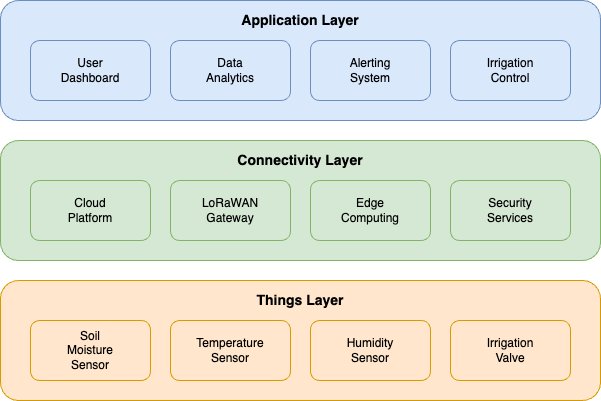
\includegraphics[width=\textwidth]{img/drawio/three_layer_architecture.png}
\caption{Three-Layer IoT Architecture for Smart Agriculture System}
\label{fig:architecture}
\end{figure}

The architecture follows a three-layer approach:

\begin{enumerate}
    \item \textbf{Things Layer}: This is the physical layer containing all the field devices.
    \begin{itemize}
        \item \textbf{Soil Moisture Sensors}: Deployed across the field to monitor moisture levels.
        \item \textbf{Temperature Sensors}: Monitor ambient and soil temperatures.
        \item \textbf{Humidity Sensors}: Track atmospheric humidity affecting evaporation rates.
        \item \textbf{Irrigation Actuators}: Valves and pumps that respond to control signals.
    \end{itemize}
    
    \item \textbf{Connectivity Layer}: This layer handles data transmission and initial processing.
    \begin{itemize}
        \item \textbf{LoRaWAN Gateway}: Collects data from all field sensors and transmits to the cloud.
        \item \textbf{Edge Computing Node}: Performs preliminary data processing and filtering.
        \item \textbf{Security Services}: Handles data encryption, device authentication, and secure communications.
        \item \textbf{Cloud Platform}: Provides storage, advanced analytics, and application hosting.
    \end{itemize}
    
    \item \textbf{Application Layer}: This layer focuses on user interaction and system control.
    \begin{itemize}
        \item \textbf{Data Analytics Engine}: Processes sensor data to derive insights and irrigation recommendations.
        \item \textbf{User Dashboard}: Web and mobile interfaces for farmers to visualize data and control the system.
        \item \textbf{Alerting System}: Generates notifications for abnormal conditions or system issues.
        \item \textbf{Irrigation Control System}: Automated decision-making for irrigation scheduling based on sensor data and analytics.
    \end{itemize}
\end{enumerate}

\begin{figure}[H]
\centering
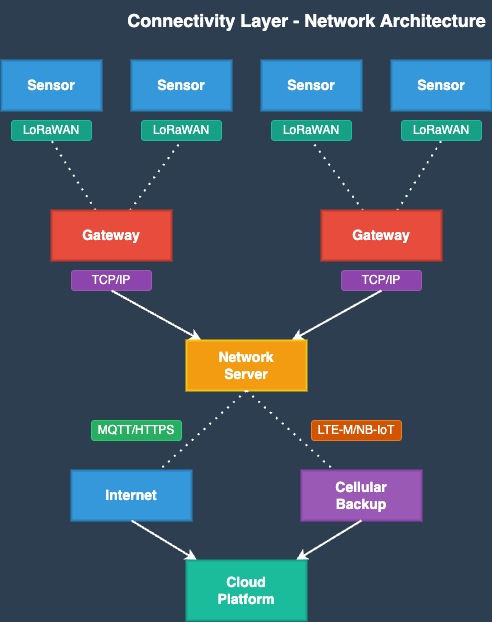
\includegraphics[width=\textwidth]{img/drawio/Connectivity_Layer.png}
\caption{Connectivity Layer - Network Architecture}
\label{fig:connectivity_layer}
\end{figure}

The three layers work together seamlessly to create a complete smart agriculture solution. The Things Layer captures environmental and soil data; the Connectivity Layer ensures this data is transmitted securely and efficiently to where it's needed; and the Application Layer transforms raw data into actionable insights and automated controls that optimize agricultural practices.

\subsubsection{Data Flow}

\begin{figure}[H]
\centering
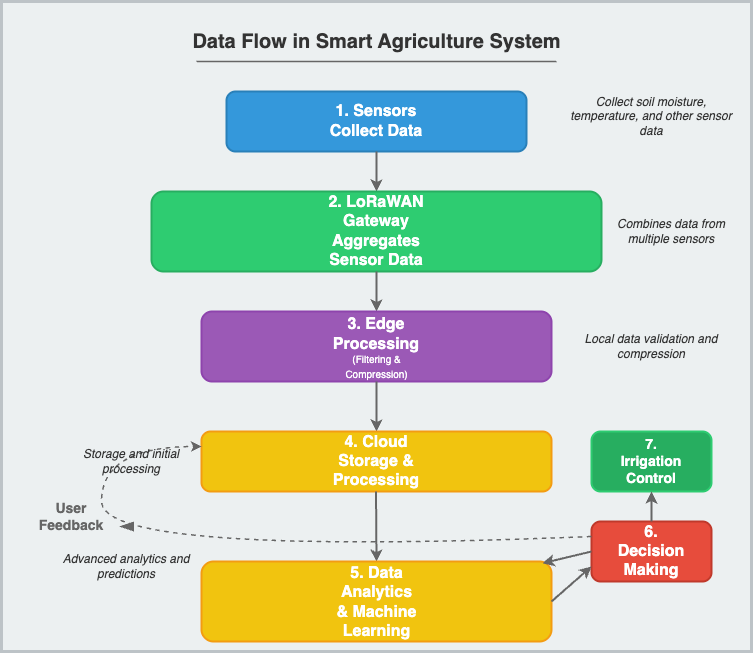
\includegraphics[width=\textwidth]{img/drawio/data_flow.png}
\caption{Data Flow in Smart Agriculture IoT System}
\label{fig:dataflow}
\end{figure}

The data flow in the system follows this pattern:

\begin{enumerate}
    \item \textbf{Data Collection}: Soil moisture sensors collect readings at regular intervals (every 30 minutes) along with temperature and humidity data.
    
    \item \textbf{Data Transmission}: The sensors transmit data to the LoRaWAN gateway using low-power, long-range communication. Each data packet includes sensor ID, timestamp, battery level, and measured values.
    
    \item \textbf{Edge Processing}: Before forwarding to the cloud, the edge computing node performs:
    \begin{itemize}
        \item Data validation to identify anomalous readings
        \item Compression to reduce bandwidth usage
        \item Preliminary analytics for urgent local decisions
    \end{itemize}
    
    \item \textbf{Cloud Storage and Processing}: The validated data is stored in a time-series database in the cloud platform. The cloud infrastructure:
    \begin{itemize}
        \item Stores historical data for trend analysis
        \item Runs complex analytics algorithms
        \item Hosts the application services
    \end{itemize}
    
    \item \textbf{Data Analytics}: The analytics engine processes the data to:
    \begin{itemize}
        \item Identify soil moisture patterns
        \item Correlate moisture with weather conditions
        \item Generate irrigation recommendations
        \item Predict future moisture levels based on weather forecasts
    \end{itemize}
    
    \item \textbf{Decision Making}: Based on analytics results, the system makes decisions about:
    \begin{itemize}
        \item When to irrigate specific zones
        \item How much water to apply
        \item Whether to override automated decisions based on user input
    \end{itemize}
    
    \item \textbf{Action Execution}: Control signals are sent back through the network to the irrigation actuators (valves and pumps) to execute the irrigation plan.
    
    \item \textbf{User Interface and Feedback}: Throughout this process, farmers can:
    \begin{itemize}
        \item View real-time soil conditions on their dashboard
        \item Receive alerts about critical conditions
        \item Override automatic decisions when necessary
        \item Analyze historical data to improve farming practices
    \end{itemize}
\end{enumerate}

\begin{figure}[H]
\centering
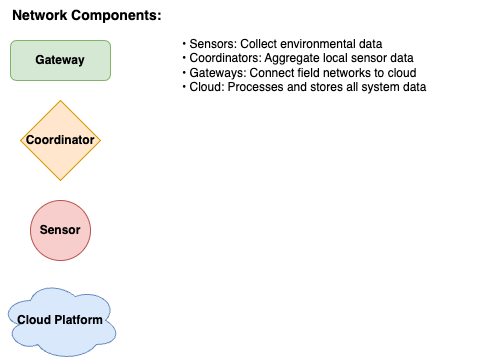
\includegraphics[width=0.7\textwidth]{img/drawio/legend.png}
\caption{Network Components Legend}
\label{fig:legend}
\end{figure}

\subsubsection{Communication Criteria}

The selection of LoRaWAN as the primary communication protocol for this smart agriculture application is based on the following criteria:

\begin{table}[H]
\centering
\begin{tabular}{@{}llll@{}}
\toprule
\textbf{Criteria} & \textbf{Requirement} & \textbf{LoRaWAN Capability} & \textbf{Justification} \\
\midrule
Range & 2-10 km & Up to 15 km rural & Agricultural fields often span large areas \\
Power Consumption & Very Low & 10+ years battery life & Remote deployment without power access \\
Data Rate & Low (100-5000 bytes/day) & 0.3-50 kbps & Moisture readings don't require high bandwidth \\
Cost & Low & Inexpensive nodes & Economic feasibility for numerous sensors \\
Infrastructure & Minimal & Single gateway for large area & Simplified deployment in rural settings \\
\bottomrule
\end{tabular}
\caption{Communication Protocol Selection Criteria}
\label{tab:communication}
\end{table}

LoRaWAN is particularly well-suited for agricultural IoT applications because:

\begin{itemize}
    \item \textbf{Range}: Agricultural fields often span large areas, and LoRaWAN's long-range capability (up to 15 km in rural areas) means fewer gateways are needed to cover the entire farm.
    
    \item \textbf{Power Efficiency}: Soil moisture sensors deployed across fields have limited access to power sources. LoRaWAN's extremely low power consumption allows sensors to operate on batteries for 5-10 years, minimizing maintenance.
    
    \item \textbf{Data Rate}: Soil moisture readings are relatively small data packages that don't require high-speed transmission. LoRaWAN's lower data rate (0.3-50 kbps) is perfectly adequate for this application.
    
    \item \textbf{Network Topology}: For larger farms, a star-of-stars topology is implemented, where multiple LoRaWAN gateways collect data from their respective areas and forward it to the cloud platform.
\end{itemize}

For local sensor-to-sensor communication and irrigation control, ZigBee is used as a secondary protocol due to its:

\begin{itemize}
    \item Lower power consumption for short-range communications
    \item Mesh network capabilities allowing sensors to relay data
    \item Higher reliability in dense sensor deployments
\end{itemize}

\subsubsection{User Interface}

\begin{figure}[H]
\centering
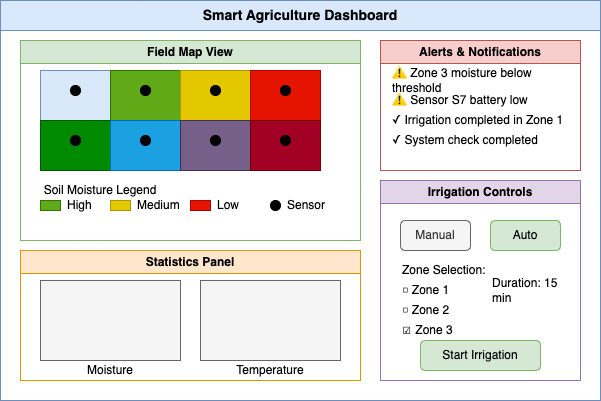
\includegraphics[width=\textwidth]{img/drawio/ui_design.png}
\caption{User Interface Design for Smart Agriculture System}
\label{fig:ui}
\end{figure}

Key features of the user interface include:

\begin{itemize}
    \item \textbf{Field Map View}: An interactive map displaying:
    \begin{itemize}
        \item Color-coded soil moisture levels across different zones
        \item Sensor locations and statuses
        \item Current irrigation activities
        \item Historical patterns through time-lapse visualization
    \end{itemize}
    
    \item \textbf{Data Visualization}:
    \begin{itemize}
        \item Real-time graphs of soil moisture, temperature, and humidity
        \item Historical trends with customizable time periods
        \item Correlation analysis between different environmental factors
        \item Weather forecast integration
    \end{itemize}
    
    \item \textbf{Alerts and Notifications}:
    \begin{itemize}
        \item Critical moisture threshold alerts
        \item System malfunction warnings
        \item Battery level indicators for sensors
        \item Irrigation schedule notifications
    \end{itemize}
    
    \item \textbf{Control Panel}:
    \begin{itemize}
        \item Manual override controls for irrigation
        \item Adjustment of moisture thresholds that trigger irrigation
        \item Scheduling tools for planned irrigation
        \item System configuration and calibration settings
    \end{itemize}
\end{itemize}

The mobile application provides essential features optimized for smartphones, focusing on alerts, quick status checks, and basic controls for on-the-go management. The web interface offers more comprehensive analytics, detailed visualization, and system configuration options, better suited for desktop use during detailed planning sessions.

\subsection{Selection of Components}

\subsubsection{Access Technology}

For this smart agriculture application, LoRaWAN has been selected as the primary access technology for the following reasons:

\begin{itemize}
    \item \textbf{Range Optimization}: Agricultural deployments require coverage over large areas, often in rural locations where cellular coverage may be limited. LoRaWAN provides excellent range (up to 15 km in line-of-sight rural conditions), allowing a single gateway to cover an entire farm in many cases.
    
    \item \textbf{Power Efficiency}: The extreme power efficiency of LoRaWAN is critical for agricultural deployments. Sensors can operate for 5-10 years on a single battery, minimizing the maintenance needs for widely distributed sensors in difficult-to-access agricultural areas.
    
    \item \textbf{Cost Effectiveness}: LoRaWAN offers a good balance between infrastructure cost and performance. The relatively low cost of end nodes (compared to cellular-based solutions) allows for dense sensor deployment, and the minimal infrastructure requirements (fewer gateways) reduce overall system costs.
    
    \item \textbf{Sufficient Data Rate}: Despite its relatively low data rate, LoRaWAN provides more than enough bandwidth for soil moisture sensing applications, which typically only need to transmit small data packages at infrequent intervals (e.g., once every 30 minutes).
    
    \item \textbf{Open Standard}: LoRaWAN is an open standard with growing ecosystem support, reducing dependency on single vendors and providing more options for components and future expansions.
\end{itemize}

\subsubsection{Topology}

\begin{figure}[H]
\centering
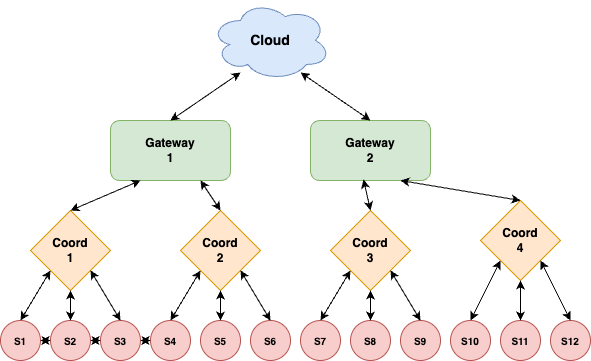
\includegraphics[width=\textwidth]{img/drawio/topology.png}
\caption{Hybrid Star-Mesh Topology for Smart Agriculture System}
\label{fig:topology}
\end{figure}

This hybrid topology has been selected for the following reasons:

\begin{itemize}
    \item \textbf{LoRaWAN Star Topology} (Upper Level):
    \begin{itemize}
        \item Simple deployment and management of the main communication backbone
        \item Efficient for long-range communication between field devices and the cloud
        \item Lower power requirements for the end devices, as they only need to reach the nearest gateway
        \item Reduced complexity of the overall network architecture
    \end{itemize}
    
    \item \textbf{ZigBee Mesh Topology} (Sensor Level):
    \begin{itemize}
        \item Enhanced reliability through multiple communication paths
        \item Ability to cover areas with challenging terrain or obstacles
        \item Elegant handling of node failures by rerouting through alternative paths
        \item Simplified expansion by adding nodes without reconfiguring the entire network
        \item Reduced transmission power for short-range communications between closely spaced sensors
    \end{itemize}
\end{itemize}

\begin{figure}[H]
\centering
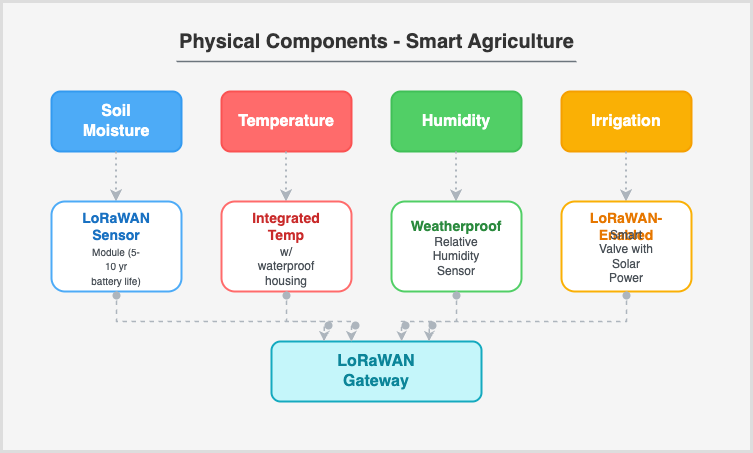
\includegraphics[width=\textwidth]{img/drawio/Physical_Components.png}
\caption{Physical Components - Smart Agriculture}
\label{fig:physical_components}
\end{figure}

The combination provides the advantages of both topologies:

\begin{itemize}
    \item Long-range communication between field zones and the central system (star)
    \item Reliable and flexible connectivity within each field zone (mesh)
    \item Optimized power usage by using the appropriate protocol for each communication distance
    \item Enhanced scalability for both expanding coverage area and increasing sensor density
\end{itemize}

\begin{figure}[H]
\centering
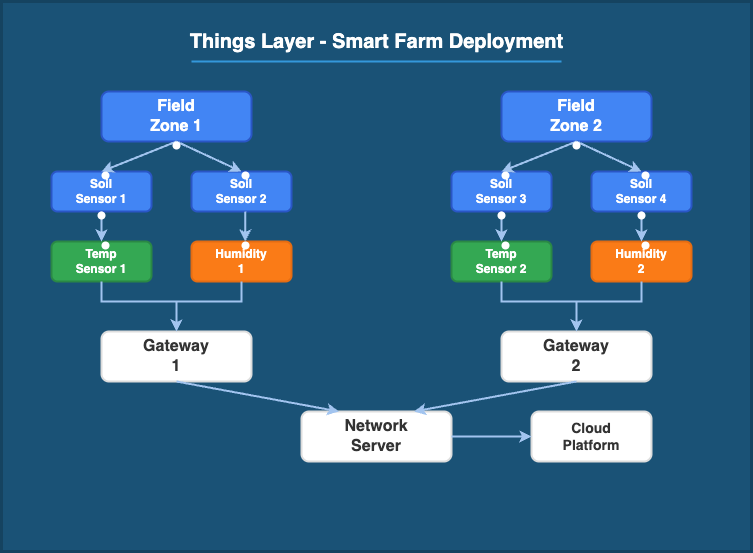
\includegraphics[width=\textwidth]{img/drawio/Things_Layer.png}
\caption{Things Layer - Smart Farm Deployment}
\label{fig:things_layer}
\end{figure}

\subsubsection{Data Management Strategy}

The data management strategy for the smart agriculture system encompasses the entire data lifecycle from collection to action:

\begin{enumerate}
    \item \textbf{Data Collection}:
    \begin{itemize}
        \item Each sensor collects soil moisture, temperature, and battery level readings at configurable intervals (default: 30 minutes)
        \item Data is timestamped and tagged with unique sensor ID and location coordinates
        \item Sensors perform basic validity checks before transmission
    \end{itemize}
    
    \item \textbf{Data Aggregation}:
    \begin{itemize}
        \item The local ZigBee network aggregates readings from nearby sensors
        \item ZigBee coordinators perform the first level of data aggregation before forwarding to LoRaWAN gateways
        \item LoRaWAN gateways collect data from all coordinators in their coverage area
    \end{itemize}
    
    \item \textbf{Data Filtering}:
    \begin{itemize}
        \item Edge devices apply filtering algorithms to detect and handle outliers
        \item Sensor readings are validated against expected ranges and historical patterns
        \item Corrupted or suspicious data points are flagged for later analysis
        \item Duplicate readings (from redundant transmission paths) are eliminated
    \end{itemize}
    
    \item \textbf{Data Compression and Transmission}:
    \begin{itemize}
        \item Data is compressed using delta encoding (storing changes rather than absolute values)
        \item Batching of multiple readings to reduce transmission overhead
        \item Prioritization of critical alerts over routine measurements
        \item Adaptive transmission rates based on detected field conditions
    \end{itemize}
    
    \item \textbf{Cloud Storage}:
    \begin{itemize}
        \item Time-series database for efficient storage and retrieval of sequential sensor data
        \item Multi-tier storage strategy (hot storage for recent data, cold storage for historical archives)
        \item Automated backup and redundancy
        \item Data partitioning by field zones for optimized query performance
    \end{itemize}
    
    \item \textbf{Data Analytics}:
    \begin{itemize}
        \item Real-time analytics for immediate irrigation decisions
        \item Batch processing for deeper historical analysis and pattern recognition
        \item Machine learning models for soil moisture prediction based on weather forecasts
        \item Correlation analysis between moisture levels, crop yield, and irrigation patterns
        \item Anomaly detection to identify sensor malfunctions or irrigation system issues
    \end{itemize}
    
    \item \textbf{Decision Support}:
    \begin{itemize}
        \item Automated threshold-based alerts for critical conditions
        \item Irrigation scheduling recommendations based on current conditions and forecasts
        \item Resource optimization algorithms to balance water conservation with crop needs
        \item Visualization tools to support farmer decision-making
    \end{itemize}
    
    \item \textbf{Data Lifecycle Management}:
    \begin{itemize}
        \item Automated data retention policies (e.g., high-resolution data for 1 month, aggregated data for 5 years)
        \item Compliance with relevant data protection regulations
        \item Data export capabilities for integration with other farm management systems
        \item Regular system audits to ensure data quality and integrity
    \end{itemize}
\end{enumerate}

This comprehensive data management strategy ensures that the smart agriculture system not only collects accurate and reliable data but also transforms it into actionable insights that drive tangible improvements in agricultural productivity and resource efficiency.

\section{Conclusion}

The IoT-based smart agriculture solution presented in this assignment demonstrates the transformative potential of modern sensing technologies and communication protocols in addressing agricultural challenges. By leveraging soil moisture sensors connected through a hybrid LoRaWAN and ZigBee network, the system provides farmers with unprecedented visibility into their field conditions and automated control over irrigation resources.

The three-layer architecture (Things, Connectivity, and Application) creates a robust framework for data collection, transmission, processing, and utilization. The selection of LoRaWAN as the primary communication protocol addresses the specific needs of agricultural deployments, particularly in terms of range, power efficiency, and cost-effectiveness. The hybrid star-mesh topology balances network reliability with power and resource constraints.

This smart agriculture implementation delivers multiple benefits including water conservation, increased crop yields, reduced labor costs, and data-driven decision-making capabilities. While challenges such as initial deployment costs, calibration requirements, and potential connectivity issues in remote areas exist, the long-term advantages significantly outweigh these limitations.

As IoT technologies continue to evolve, future enhancements could include integration with drone-based imaging, advanced soil nutrient sensors, and more sophisticated machine learning algorithms to further optimize agricultural practices. The modular architecture of the system allows for such expansions, ensuring the solution remains valuable and adaptable to changing agricultural needs.

\section{References}

\begin{enumerate}
    \item Al-Sarawi, S., Anbar, M., Alieyan, K., \& Alzubaidi, M. (2023). Internet of Things (IoT) communication protocols: Review. \textit{IEEE Sensors Journal, 23}(5), 4–15.
    
    \item Tzounis, A., Katsoulas, N., Bartzanas, T., \& Kittas, C. (2023). Internet of Things in agriculture, recent advances and future challenges. \textit{Biosystems Engineering, 164}, 31–48.
    
    \item Kamienski, C., Soininen, J. P., Taumberger, M., Dantas, R., Toscano, A., Salmon Cinotti, T., Filev Maia, R., \& Torre Neto, A. (2023). Smart water management platform: IoT-based precision irrigation for agriculture. \textit{Sensors, 19}(2), 276.
    
    \item Li, D., Zheng, Y., \& Zhao, W. (2024). LoRaWAN for Smart Agriculture: A Comparative Study of Communication Technologies. \textit{IEEE Access, 12}, 112876–112885.
    
    \item Farooq, M. S., Riaz, S., Abid, A., Umer, T., \& Zikria, Y. B. (2023). Role of IoT technology in agriculture: A systematic literature review. \textit{Electronics, 12}(3), 522.
    
    \item Hasan, M., Islam, M., Zarif, M., \& Hashem, M. (2024). Internet of Things based smart farming system using LoRaWAN. \textit{IEEE Journal on Internet of Things, 1}(2), 102–112.
    
    \item Zhang, N., Wang, M., \& Wang, N. (2023). Precision agriculture—a worldwide overview. \textit{Computers and Electronics in Agriculture, 36}(2–3), 113–132.
\end{enumerate}

\end{document}